
%(BEGIN_QUESTION)
% Copyright 2010, Tony R. Kuphaldt, released under the Creative Commons Attribution License (v 1.0)
% This means you may do almost anything with this work of mine, so long as you give me proper credit

Suppose someone builds a dual-junction thermocouple circuit using type T thermocouple wire (copper and constantan metals), then measures voltage between the two junctions with a voltmeter:

$$\includegraphics[width=15.5cm]{i03172x01.eps}$$

Calculate the voltage read by the voltmeter, using a type T thermocouple table to find millivolt potentials for each of the junctions.

\underbar{file i03172}
%(END_QUESTION)





%(BEGIN_ANSWER)

The voltmeter should read -0.643 millivolts, because the 105 $^{o}$F junction has a potential of 1.635 millivolts, the 77 $^{o}$F junction has a potential of 0.992 millivolts, and the two junctions' voltages are {\it opposing} one another in polarity with the positive terminal of the voltmeter connected to the negative-most copper wire.

%(END_ANSWER)





%(BEGIN_NOTES)


%INDEX% Measurement, temperature: thermocouple

%(END_NOTES)


